\documentclass[8pt,final,xcolor={usenames,x11names}]{beamer}
\usepackage[usenames,x11names]{xcolor,colortbl}

\usepackage[utf8]{inputenc}
\usepackage{default}
\usepackage{hyperref}
\usepackage{textpos}
\usepackage{verbatimbox}
\usetheme{Copenhagen}

\title{Identity chain management for banks: law 7.8.2009/617}
\subtitle{``Laki vahvasta sähköisestä tunnistamisesta ja sähköisistä luottamuspalveluista''\\17 §: ``Tunnistusvälineen hakijana olevan luonnollisen henkilön tunnistaminen''}
\author{Tero Keski-Valkama}
\institute{
\includegraphics[height=1.4cm]{CybercomG_logo_Classic_RGB.png}}
\date{2017-11-22}

\addtobeamertemplate{frametitle}{}{%
\begin{textblock*}{100mm}(10.95cm,-0.8cm)

\includegraphics[height=0.8cm]{cybercom-blue.png}
\end{textblock*}}


\begin{document}

\frame{\titlepage}
 
\begin{frame}
\frametitle{Why?}

\begin{itemize}
 \item The law for electronic identification includes the 17 § which allows banks to perform the first identification of a new customer using an electronic strong identification method.
       In practice this means identification through electronic identification performed by another bank.
 \item The text of the relevant part of the law: ``Olemassa olevan vahvan sähköisen tunnistusvälineen avulla on voitava hakea vastaavan tasoista sähköistä tunnistusvälinettä. Aiempaan tunnistukseen luottava vahvan sähköisen tunnistuspalvelun tarjoaja vastaa mahdollisesta tunnistuksen virheellisyydestä suhteessa vahingon kärsineeseen.''
 \item So, what happens if a criminal uses a stolen strong authentication of user X in bank A to create an account in another bank B?
 \item The consumer reports the credentials as stolen to bank A, and bank A revokes the credentials. What happens to the new credentials in bank B?
 \item Cybercom and blockchain to the rescue! Let's store all the identity related actions in an unmodifiable, shared log.
\end{itemize}

\end{frame}

\begin{frame}
\frametitle{Background – Guardtime Keyless Signature Infrastructure}

\begin{itemize}
 \item Guardtime KSI offers a convenient service component for establishing specific kinds of guarantees regarding trust.
 \item In practice KSI can be used to prove that a specific document has existed at a specific point of time, by storing the hash digest of the document in an unmodifiable hash calendar (merkle tree).
 \item Guardtime only receives the hash digest of the document, never the whole document.
 \item In Cybercom Identity Chain proposal Guardtime KSI is used to offer additional guarantees that the shared identity event log is unmodifiable.
\end{itemize}

\end{frame}

\begin{frame}
\frametitle{Background – IBM Hyperledger Fabric}

\begin{itemize}
 \item In addition to hash digests, we will also need to store the master data in a manner that is robustly available to all cooperating banks.
 \item IBM Hyperledger Fabric is a platform for implementing consortium blockchains.
 \item As opposed to public blockchains like Ethereum, consortium blockchains do not require an associated cryptocurrency and they require a trusted party that manages consortium memberships.
 \item Storing a shared registry of identity events in a consortium blockchain makes it unmodifiable after once written, and available to all cooperating parties.
\end{itemize}

\end{frame}

\begin{frame}
\frametitle{Architecture}

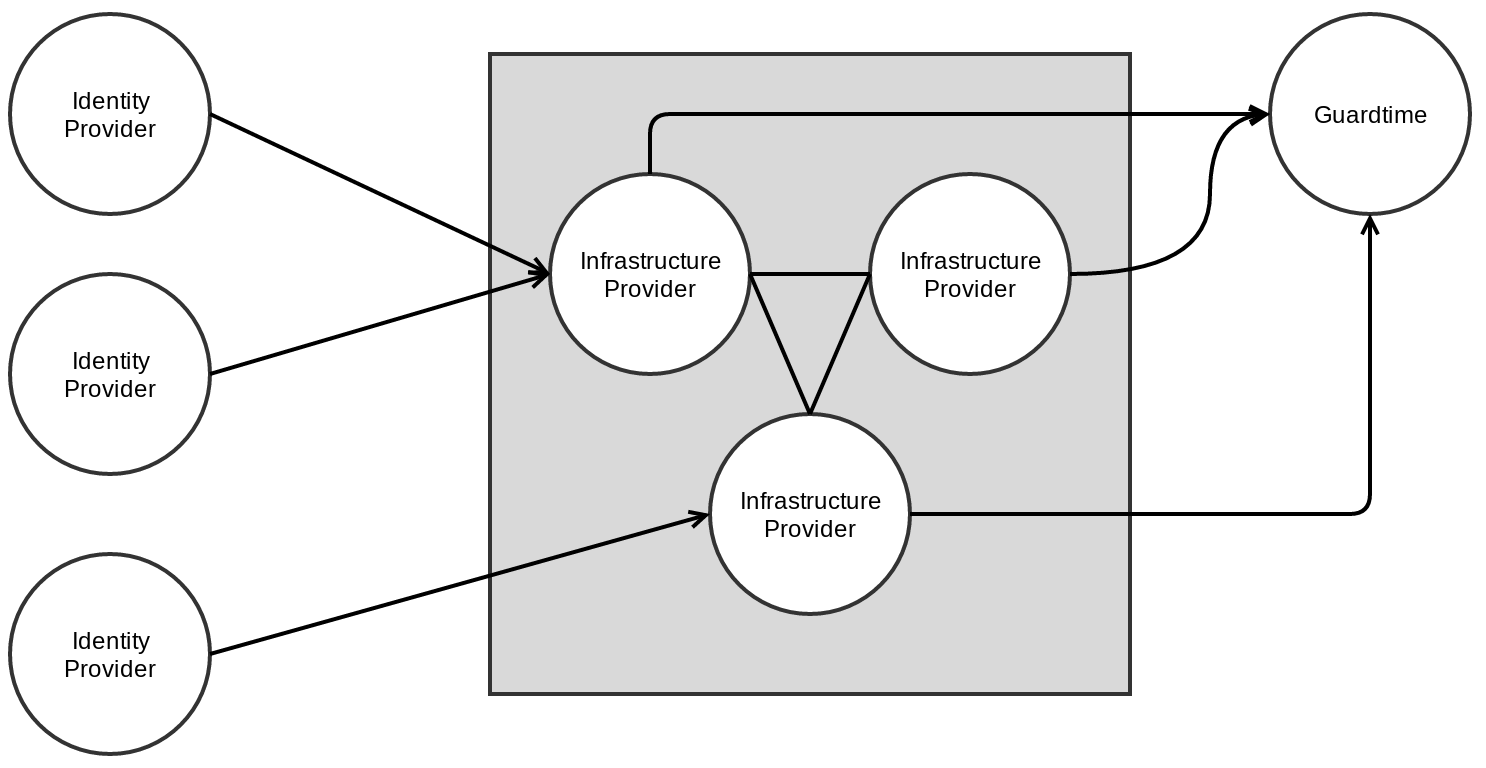
\includegraphics[width=0.9\textwidth]{./deployment.png}

\begin{itemize}
 \item Banks can work as infrastructure providers and/or identity providers in the architecture.
\end{itemize}

\end{frame}

\begin{frame}[fragile]
\frametitle{Operation}
\begin{enumerate}
 \item Person A has their identity for \colorbox{PaleTurquoise1>wheel,1,5}{Bank X} stolen
 \item \colorbox{PaleTurquoise1>wheel,1,5}{Stolen identity (X)} used to create a new account in \colorbox{PaleTurquoise1>wheel,2,5}{Bank Y}
 \item Person A \underline{retroactively} revokes their identity at \colorbox{PaleTurquoise1>wheel,1,5}{Bank X}
 \item \colorbox{PaleTurquoise1>wheel,2,5}{Fake identity (Y)} used to create a new account in \colorbox{PaleTurquoise1}{Bank Z}
 \item \colorbox{PaleTurquoise1}{Fake identity (Z)} used in criminal activity
\end{enumerate}
\begin{itemize}
 \item If \colorbox{PaleTurquoise1}{Bank Z} did not check the identity chain state in blockchain at (4), then \colorbox{PaleTurquoise1}{Bank Z} is liable for damages.
 \item If \colorbox{PaleTurquoise1}{Bank Z} did check, but \colorbox{PaleTurquoise1>wheel,1,5}{Bank X} did not correctly mark this revocation in time to the blockchain to prevent (4), then \colorbox{PaleTurquoise1>wheel,1,5}{Bank X} is liable.
 \item If \colorbox{PaleTurquoise1>wheel,1,5}{Bank X} marked the revocation and \colorbox{PaleTurquoise1}{Bank Z} checked the chain status, then (4) failed and (5) did not happen.
 \item Liability is based on consortium membership contract. Blockchain provides an indisputable log of events to determine liability.
 \item \emph{Alternative: 3 banks in court, none of which trusts each other's IT systems or logs, with a 20 million euro money laundering case.}
\end{itemize}

\end{frame}
\end{document}

